\section{Completed experiments}
All numbers are produced by the code in this project (\texttt{results/*.json}); sandbox: 2 CPU cores, no GPU. Test sets are fixed and independent of every generator: 800 everyday scenarios, 800 hazard scenarios (collide if the ego does not react), and the hard-perception subset (\nHard\ scenarios with dropout $>0.4$ or radius $>0.6$\,m).

\subsection{E1: Learned policy and diffusion-generated edge cases}\label{sec:e1}
\textbf{Setup.} Four DAgger policies on 2\,700 scenarios each, \nSeeds\ seeds: A everyday only; B +\nGen\ guided diffusion; C +\nGen\ unguided diffusion; D +\nGen\ uniform random.
\begin{table}[H]\centering\small
\begin{tabular}{lcccc}\toprule
 & \multicolumn{3}{c}{Collision rate [\%]} & Hazard\\\cmidrule(lr){2-4}
Training data & Everyday & Hazard & Hard-perception & min.\ gap [m]\\\midrule
A everyday only & $\collAnormal$ & $\collAhazard$ & $\collAhard$ & $\gapAhazard$\\
B + guided diffusion & $\collBnormal$ & $\collBhazard$ & $\collBhard$ & $\gapBhazard$\\
C + unguided diffusion & $\collCnormal$ & $\collChazard$ & $\collChard$ & $\gapChazard$\\
D + uniform random & $\collDnormal$ & $\collDhazard$ & $\collDhard$ & $\gapDhazard$\\\midrule
Privileged expert & $\expertnormal$ & $\experthazard$ & $\experthard$ & $\expertgap$\\\bottomrule
\end{tabular}
\caption{Mean $\pm$ std over \nSeeds\ seeds.}
\end{table}
\begin{figure}[H]\centering
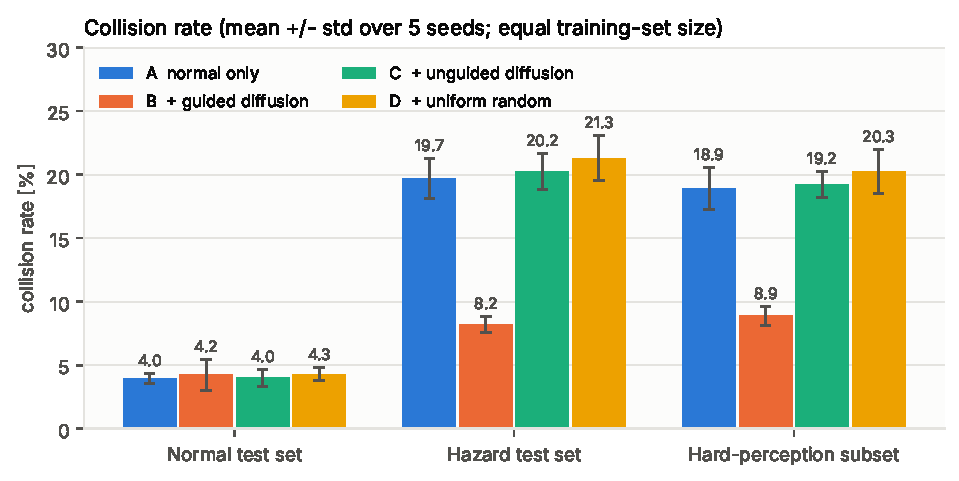
\includegraphics[width=0.88\linewidth]{exp_collision_rates}\\[2pt]
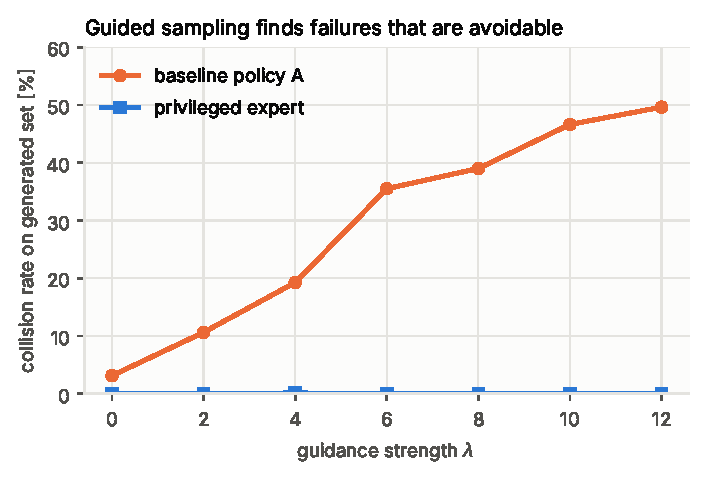
\includegraphics[width=0.48\linewidth]{exp_guidance_sweep}\hfill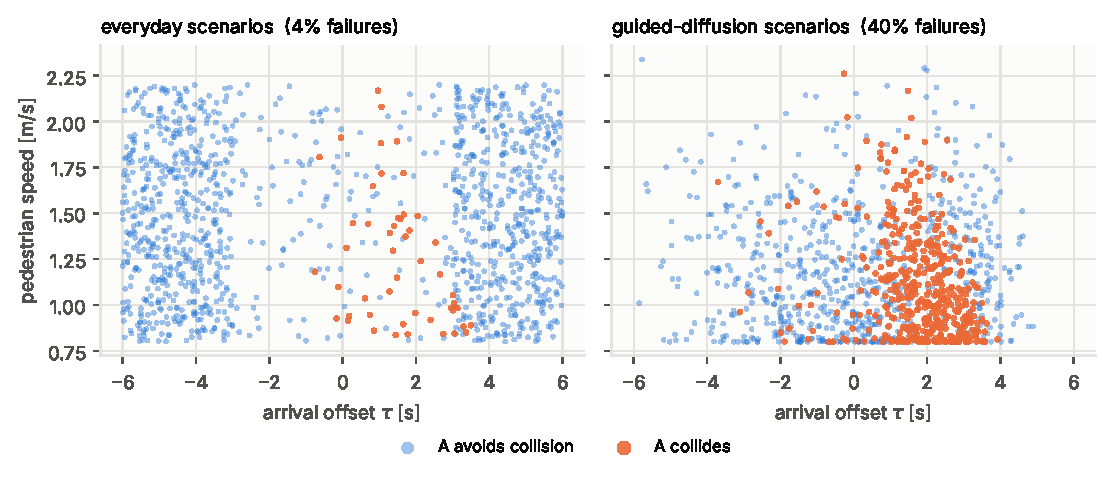
\includegraphics[width=0.5\linewidth]{exp_scatter}
\caption{Top: collision rates. Bottom left: guidance strength $\lambda$ versus failures of policy A on generated sets. Bottom right: where A fails (seed 0).}
\end{figure}
\textbf{Observations.} Only guided data helps ($\collAhazard\to\collBhazard\%$ on hazards); unguided or uniform data of the same size does not (C, D within seed noise of A). Guided scenarios are hard for A (\diagguidedAcoll\% collide) but avoidable (expert \diagguidedExcoll\%). Everyday performance and completion are unchanged. Remaining failures are perception-limited.

\subsection{E2: NeRF-style digital twin}\label{sec:e2}
\textbf{Setup.} 10 expert drives logged (\nerfRays\ rays), field trained \nerfIters\ iterations (\nerfFit\,s); evaluation on 2 unseen drives and on a closed-loop what-if grid (13 pedestrian shifts $\times$ 4 ego speeds) run both in the twin and in the real simulator.
\begin{table}[H]\centering\small
\begin{tabular}{lr}\toprule
Metric & Value\\\midrule
Mean abs.\ range error, held-out views, all rays [m] & $\nvMAE$ (static-only field: $\nvMAEstatic$)\\
Rays within 0.5\,m & $\nvWithin\%$\\
Pedestrian-hit rays ($\nvPedRays$ of $\nvAllRays$): error [m] & $\nvMAEped$ (static-only: $\nvMAEstaticped$)\\
What-if collision outcome agreement ($\wiNcfg$ cases) & $\wiAgree\%$\\
Collision rate real / twin & $\wiCollReal\%$ / $\wiCollTwin\%$\\
Min-gap correlation real vs.\ twin; mean abs.\ difference [m] & $\wiGapCorr$; $\wiGapMAE$\\
Twin without dynamic field: collision rate & $\wiCollNoPed\%$\\\bottomrule
\end{tabular}
\caption{Twin fidelity.}
\end{table}
\begin{figure}[H]\centering
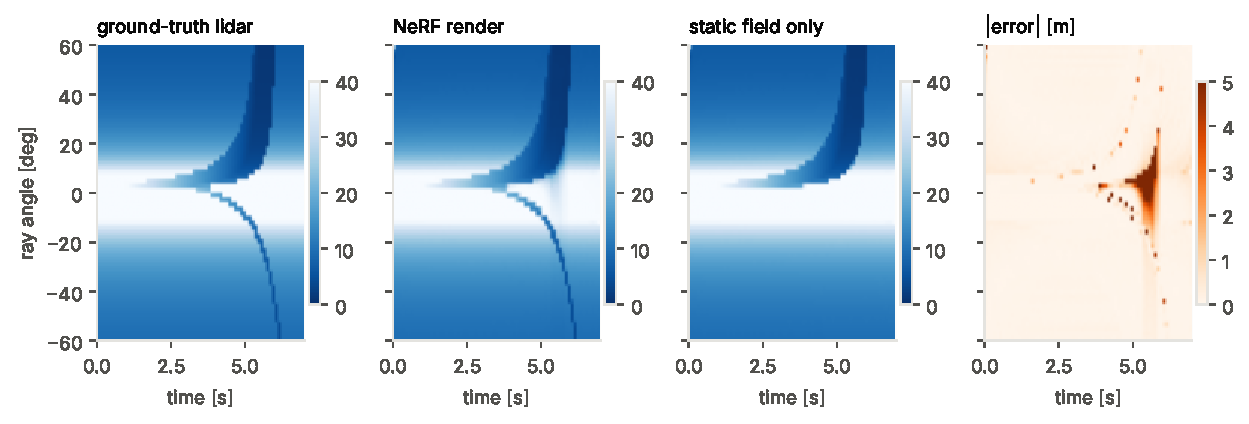
\includegraphics[width=\linewidth]{twin_range_images}\\[2pt]
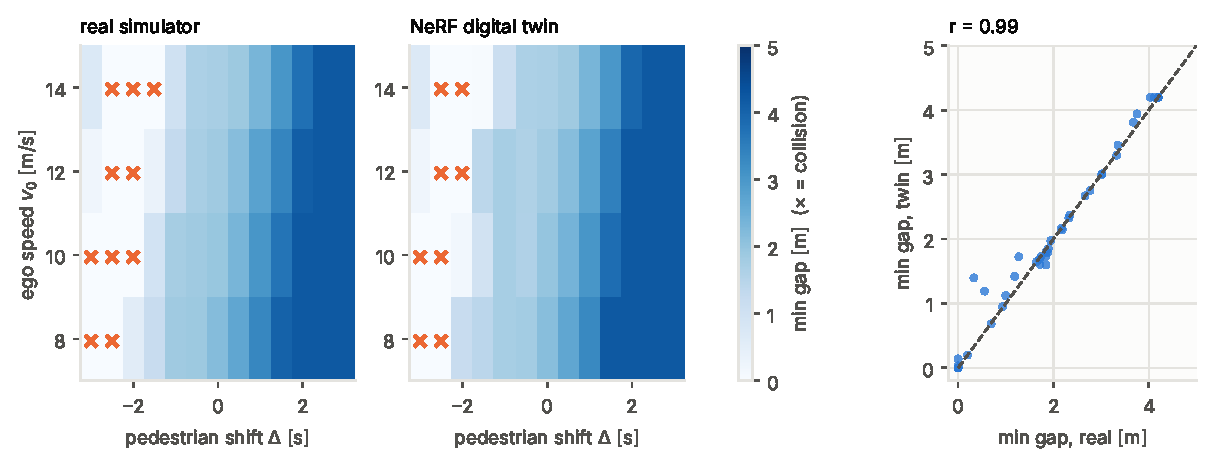
\includegraphics[width=\linewidth]{twin_whatif}
\caption{Top: held-out range images (ground truth, render, static-only, error). Bottom: what-if grid, real simulator versus twin ($\times$ = collision).}
\end{figure}
\textbf{Observations.} The dynamic component is essential: without it the pedestrian is invisible and the policy collides $\wiCollNoPed\%$ of the time. The twin misses fine detail on pedestrian rays (the error panel shows the largest errors late in the drive, when the pedestrian is close to the ego) and reproduces only the logged pedestrian trajectory, shifted in time.

\subsection{E3: Behaviour-tree verification}\label{sec:e3}
\begin{table}[H]\centering\small
\begin{tabular}{ll}\toprule
Property (checked in every abstract state) & Result\\\midrule
P1 action defined and within actuator limits & all hold\\
P2 emergency $\Rightarrow$ full braking $-a_b$ & all hold\\
P3 must-brake $\Rightarrow$ $a\in[-a_b,-0.3]$ & all hold\\
P4 conflict $\Rightarrow$ never accelerate & all hold\\
P5 no conflict $\Rightarrow$ $a\in[-3,2.5]$ & all hold\\
P6 acceleration non-increasing in hazard level & all hold\\\bottomrule
\end{tabular}
\caption{Exhaustive check over $\treeStates$ abstract states (counts per property in \texttt{results/stack.json}).}\label{tab:tree}
\end{table}
\begin{table}[H]\centering\small
\begin{tabular}{llr}\toprule
Tree version & Change & Violations in $\bmcN$\\\midrule
v1 & initial (margins 0/0.5\,s, curb pedestrian assumed safe) & 78 (\texttt{logs/design\_iteration\_1.log})\\
v2 & timing margins only (0.5/1.0\,s) & 276$^\dagger$\\
v3 & + ``yield'' level (never accelerate in conflict) & 78$^\dagger$\\
v4 & + curb pedestrian may start at 3.5\,m/s & 1$^\dagger$\\
v5 (final) & + margins 0.3/0.8\,s & $\bmcViol$ (\texttt{results/stack.json})\\\bottomrule
\end{tabular}
\caption{Bounded model check with true pedestrian state. $^\dagger$Interactive intermediate runs, not archived as files. Of the 78 counterexamples of v1, 75 had a 3.5\,m/s pedestrian: the tree accelerated towards a pedestrian waiting at the curb and could not stop when it started running.}
\end{table}
\textbf{Observation.} Model checking found a real design flaw that unit tests on everyday data had not. Adding margins alone made it worse, which shows the check is not trivially satisfied. The result covers a finite grid with ideal perception only.

\subsection{E4: Planner, optimisation and tracking}\label{sec:e4}
\textbf{Setup.} First 100 hazard scenarios, same lidar perception for BT and planner.
\begin{table}[H]\centering\small
\begin{tabular}{lccc}\toprule
Controller & Collision [\%] & Completed [\%] & Mean min.\ gap [m]\\\midrule
Learned policy A (seed 0) & $\stackAColl$ & $\stackAPass$ & ---\\
Behaviour tree, lidar perception & $\stackBTColl$ & $\stackBTPass$ & $\stackBTGap$\\
Behaviour tree, true pedestrian state & $\stackBToColl$ & $\stackBToPass$ & $\stackBToGap$\\
Lattice + optimiser + PD & $\stackPlColl$ & $\stackPlPass$ & $\stackPlGap$\\
Lattice + optimiser + PD + BT supervisor & $\stackPsColl$ & $\stackPsPass$ & $\stackPsGap$\\\bottomrule
\end{tabular}
\caption{Closed-loop comparison. On all 800 hazard / 800 everyday scenarios the BT with lidar collides in $\btFullHz\%$ / $\btFullNorm\%$.}
\end{table}
\begin{table}[H]\centering\small
\begin{tabular}{lcccc}\toprule
60 hazard scenarios, planner only & RMS tracking error [m] & Collision [\%] & 95th pct.\ jerk [m/s$^3$]\\\midrule
Feed-forward only, nominal brakes & $\trFFRms$ & $\trFFColl$ & $\trFFJerk$\\
PD + feed-forward, nominal brakes & $\trPDRms$ & $\trPDColl$ & $\trPDJerk$\\
Feed-forward only, brake gain 0.8 & $\trFFmRms$ & $\trFFmColl$ & $\trFFmJerk$\\
PD + feed-forward, brake gain 0.8 & $\trPDmRms$ & $\trPDmColl$ & $\trPDmJerk$\\
PD + feed-forward, no optimisation & --- & $\nsColl$ & $\nsJerk$\\\bottomrule
\end{tabular}
\caption{Tracking and optimisation ablations.}
\end{table}
\begin{figure}[H]\centering
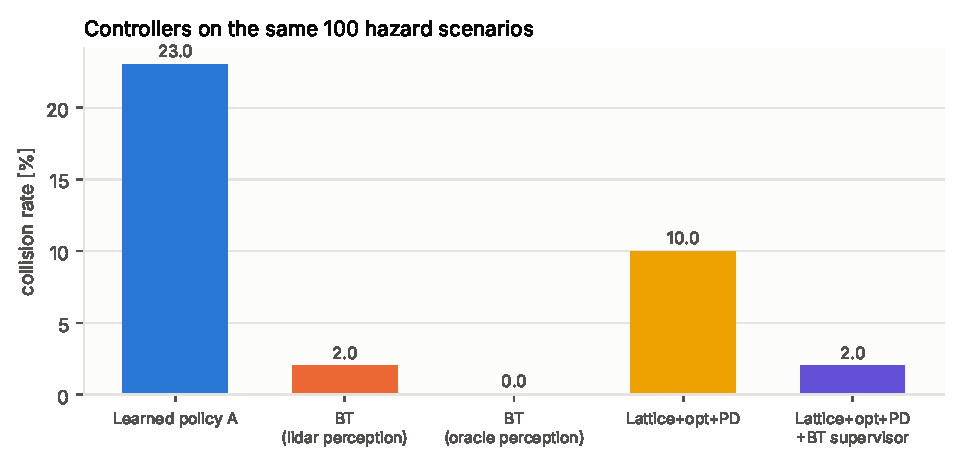
\includegraphics[width=0.62\linewidth]{stack_compare}\\[2pt]
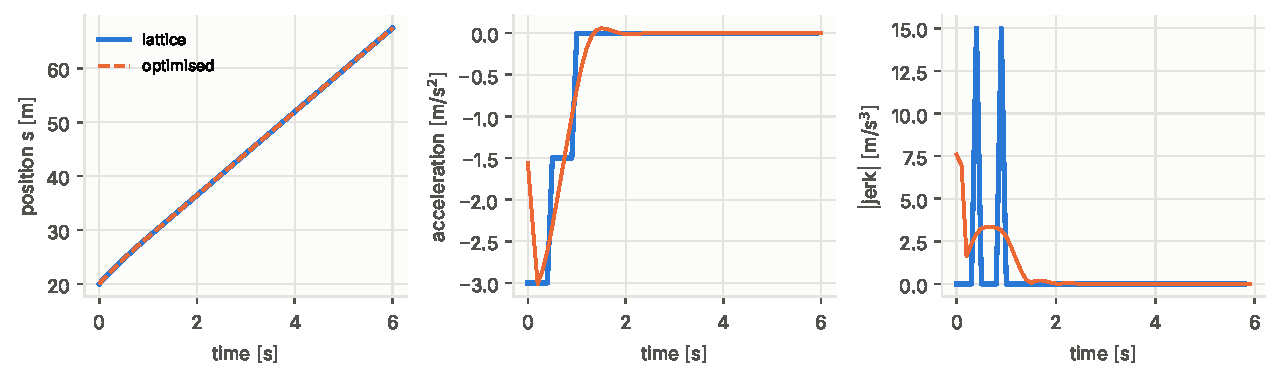
\includegraphics[width=\linewidth]{stack_trajectory}
\caption{Top: controllers on the same scenarios. Bottom: one lattice path versus its optimised refinement (position, acceleration, jerk).}
\end{figure}
\textbf{Observations.} (i) The lattice planner alone collides more than the BT because its pedestrian estimate lags a sudden start; the BT supervisor removes most of this at similar completion. (ii) Optimisation reduces the mean per-plan peak jerk from $\pljerklat$ to $\pljerksm$\,m/s$^3$, but the executed 95th-percentile jerk is essentially unchanged ($\trPDJerk$ with versus $\nsJerk$ without optimisation): replanning every 0.5\,s restarts the profile and the PD term adds step changes, so the smoothing benefit does not reach the vehicle in this configuration. (iii) PD feedback gave no measurable benefit over feed-forward: replanning at 2\,Hz re-anchors the reference to the measured state, so tracking error stays near 6--7\,cm either way; the collision differences in the table are within noise for 60 scenarios. (iv) The learned policy is worst, as in E1.

\subsection{E5: Fault injection}\label{sec:e5}
\begin{table}[H]\centering\small
\begin{tabular}{lcc}\toprule
Fault (400 hazard scenarios) & BT collisions [\%] & BT + monitor [\%]\\\midrule
None (nominal) & $\fNoneplain$ & $\fNonemonitor$\\
Lidar dropout (2\,s) & $\fdropoutplain$ & $\fdropoutmonitor$\\
Frozen frame (2\,s) & $\fstuckplain$ & $\fstuckmonitor$\\
Range bias $\times1.25$ & $\fbiasplain$ & $\fbiasmonitor$\\
Latency 0.3\,s & $\flatencyplain$ & $\flatencymonitor$\\
Brake fade to $-4$\,m/s$^2$ & $\fbrakeplain$ & $\fbrakemonitor$\\\bottomrule
\end{tabular}
\caption{Single-fault injection, lidar perception.}
\end{table}
\begin{figure}[H]\centering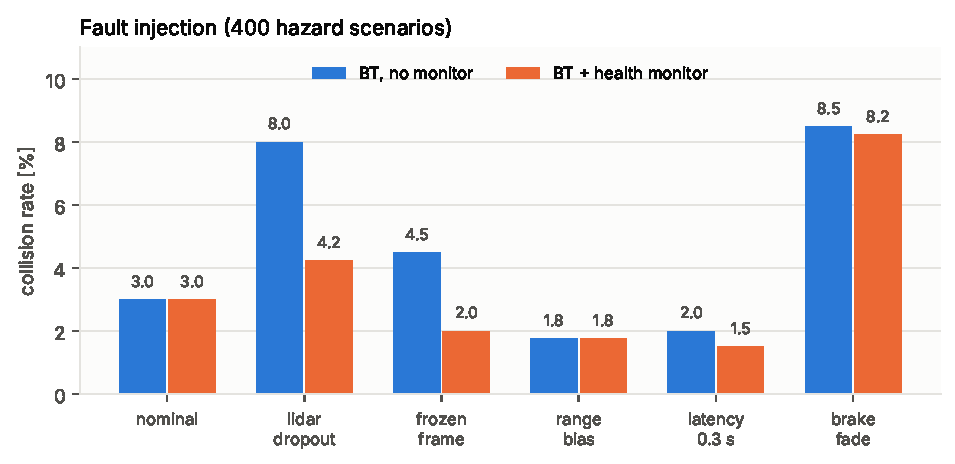
\includegraphics[width=0.82\linewidth]{stack_faults}\caption{Fault injection results.}\end{figure}
\textbf{Observations.} With 400 scenarios the standard error at a 3\% rate is about 0.9 percentage points, so differences below roughly 2 points are not significant. The monitor clearly helps for lidar dropout and frozen frames (about halving collisions). Range bias and latency of this size showed no harmful effect. Brake fade is the one fault that raises collisions markedly, and the monitor does not help: it detects fade only after the first hard braking, which is too late. This is recorded as a residual hazard.

\subsection{E6: Embedded deployment (host CPU)}\label{sec:e6}
\begin{table}[H]\centering\small
\begin{tabular}{lcc}\toprule
Policy ($\embParams$ parameters, $\embMacs$ MACs) & float32 & int8 weights\\\midrule
Latency per inference, gcc -O2, host CPU [\textmu s] & $\embFlns$ & $\embIqns$\\
Code + weights, gcc -Os [KiB] & $\embFlflash$ & $\embIqflash$\\
Max.\ abs.\ difference to NumPy output [m/s$^2$] & \embFlerr{} & \embIqerr{}\\
Collision rate, everyday / hazard set [\%] & $\embFln$ / $\embFlh$ & $\embIqn$ / $\embIqh$\\\bottomrule
\end{tabular}
\caption{C export. Host timings are not microcontroller timings.}
\end{table}
\textbf{Observations.} The generated C reproduces the NumPy policy to float rounding. int8 weights cut code+weights size to about a quarter at a small accuracy cost on hazards; latency is not better on the host because the loop converts int8 to float. On-target cycles are not measured (Sec.~\ref{sec:planned}).

\subsection{E7: Dataset adapter (software test only)}\label{sec:e7}
\texttt{datasets.py} turns KITTI tracking labels into scenario vectors (crossing speed, distance, arrival offset $\tau$). It passes a unit test on a synthetic KITTI-format track with known speed (\texttt{tests.py}). It has \emph{not} been run on real KITTI, nuScenes or Waymo data, which are not reachable from the sandbox.
